\documentclass[conference]{IEEEtran}
\IEEEoverridecommandlockouts
% The preceding line is only needed to identify funding in the first footnote. If that is unneeded, please comment it out.

\usepackage{amsmath,amssymb,amsfonts}
\usepackage{algorithmic}
\usepackage{graphicx}
\usepackage{textcomp}
%\usepackage{xcolor}
\usepackage{multirow}
\usepackage{caption}
\usepackage{subcaption}
\usepackage{booktabs}
\usepackage[table,xcdraw]{xcolor}

\def\BibTeX{{\rm B\kern-.05em{\sc i\kern-.025em b}\kern-.08em
    T\kern-.1667em\lower.7ex\hbox{E}\kern-.125emX}}
\begin{document}

\title{YOUR TITLE \\ {\large SUBTITLE}
\thanks{THANKS MESSAGE IF ANY}
}

\author{\IEEEauthorblockN{Author One}
\IEEEauthorblockA{School of Electrical and\\
Computer Engineering\\
Georgia Institute of Technology\\
Atlanta, Georgia 30332--0250\\
Email: mshell@ece.gatech.edu}
\and
\IEEEauthorblockN{Homer Simpson}
\IEEEauthorblockA{Twentieth Century Fox\\
Springfield, USA\\
Email: homer@thesimpsons.com}
\and
\IEEEauthorblockN{James Kirk\\
and Montgomery Scott}
\IEEEauthorblockA{Starfleet Academy\\
San Francisco, California 96678-2391\\
Telephone: (800) 555--1212\\
Fax: (888) 555--1212}}

\maketitle

\begin{abstract}
Determining a network baseline is one important metric for achieving situational awareness on an enterprise network, yet this task is often left undone. Further, defense organizations need to differentiate normal network traffic patterns in support of comprehensive cyberspace operations but lack a pre-operational baseline upon which to compare. This is predominantly due to the fact that a properly established baseline requires the collection of network packet capture and performance metrics, optimally, prior to network deployment. Compounding the issue, the volume and voracity of network traffic requiring analysis is increasing, making the application of Deep Packet Inspection (DPI) technologies more infeasible \cite{epstein_2017}\cite{doi:10.1137/1.9781611972733.3}.

Using features of network flow metadata, we propose a method for producing a generalizable baseline to support operational analysis on established networks. By first decomposing network traffic into a feature space based on predictive importance, we can observe these collected features and identify patterns over time in order to enable anomaly detection \cite{1212675}.  Using linear regression, we attempt network packet classification as the first step in a hierarchical approach to be expanded and tested as part of future work.
\end{abstract}

\begin{IEEEkeywords}
cyber security, network security, network baseline, machine learning, linear regression, packet classification
\end{IEEEkeywords}  

\section{Introduction}
\subsection{Network Baselining: Measured vs Relative}
First, this paper makes a distinction between a Measured Network Baseline and a Relative Network Baseline.  A Measured Network Baseline is a ``true'' baseline in a traditional sense, as a series of objective measurements on the performance and behavior of a computer network \cite{cisco_2017}, ideally conducted prior to the moment users begin to utilize the network in order to properly capture the autonomic events and activities occurring on the network by simply existing (vulnerability scans, DNS resolution queries, load balancing, etc.) \cite{1212675}. It is from this baseline that network security professionals attempt to filter out the every day workings of a network from the anomalous behaviors which they hope to detect. However many extant networks have not been baselined, and more importantly change over time. The approach in this paper is to introduce the concept of a Relative Network Baseline by identifying means and methods to which conduct baseline measurements on existing operating networks by recording network traffic, extrapolating and describing ``normal'' behaviors with machine learning and statistical methods, and create models of this behavior.

We do acknowledge certain challenges and assumptions in this approach. Accuracy of any baseline on a preexisting network could naturally be impeded by several factors: incomplete accounting of network devices, the presence of an adversary or Advanced Persistent Threat (APT) on the network, a lack of representative data due to volume or time, as well as benign abnormal host activity.  However, even with the drawbacks of a performing a relative baseline, it is our position that valuable insights can still be achieved.

\subsection{Dataset}
The body of this work was conducted in the Lincoln Research Network Operations Center (LRNOC) within MIT Lincoln Laboratory, having access to over five years of network flow data upon which to conduct analysis. Metadata was collected through a RESTful API to the network traffic and flow records and aggregated at 30 second intervals. The standard network five-tuple was collected in addition to two more features available by virtue of the aggregation:

\begin{table}[htbp]
\centering
\caption{Dataset Features}
\label{tab:dataset}
\begin{tabular}{|c|c|c|c|c|c|c|}
\hline
\multirow{2}{*}{Time} & \multicolumn{2}{c|}{IP} & \multicolumn{2}{c|}{Port} & \multicolumn{2}{c|}{Aggregated} \\ \cline{2-7} 
 & Src & Dst & Src & Dst & Payload & Packets \\ \hline
\end{tabular}
\end{table}

The aggregated process yields the total payload size (in bytes) as well as the number of packets transferred between unique IP and Port pairs within the user-selected interval size (in this case, 30 seconds). For the purposes of this paper, we further loosely define ``sessions'' as unique, directional flows within the user-selected time interval.

\subsection{Exploration Activity}

\begin{figure*}
	\centering
	\begin{subfigure}{9cm}
	\centering
	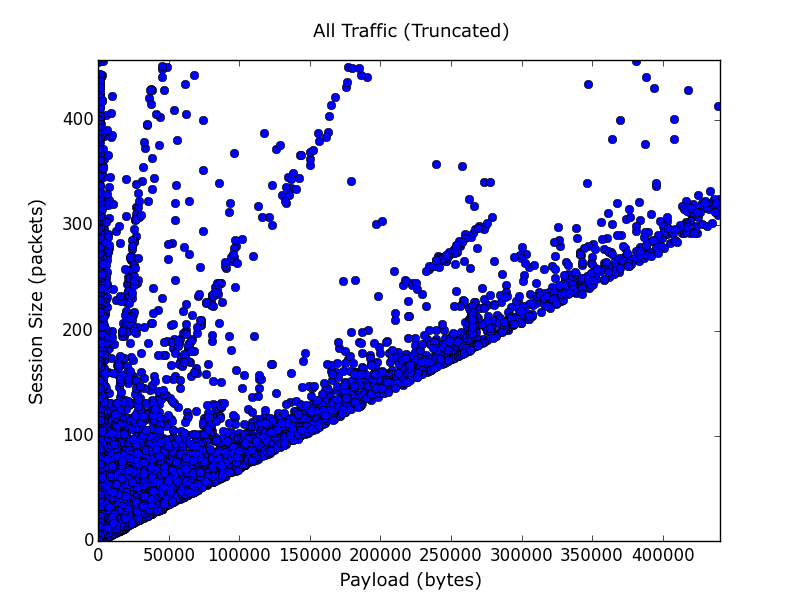
\includegraphics[width=\linewidth]{paperplots/everything.png}
	\label{subfig:all_traffic}
	\caption{Linear clustering within the dataset (zoomed)}
	\end{subfigure}%
	\begin{subfigure}{9cm}
	\centering
	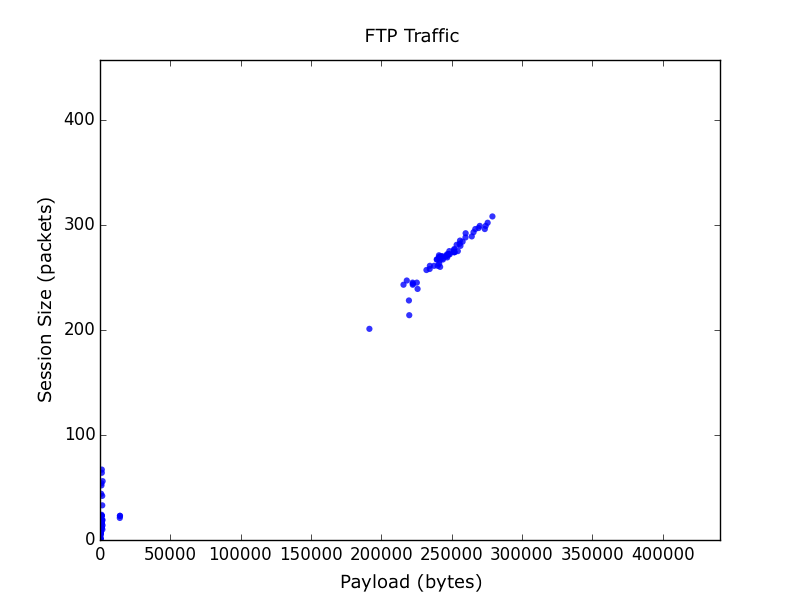
\includegraphics[width=\linewidth]{paperplots/ftp.png}
	\label{subfig:ftp}
	\caption{Manually verified cluster of FTP traffic, isolated from Sub. (a)}
	\end{subfigure}
	\caption{Exploration activity using manual analysis methods}
	\label{fig:explore}
\end{figure*}


Our efforts consider the linear relationship between the number of packets transmitted in a single session versus the amount of data passed within the payload (or content) of the communication. In this sense, one should be able to ultimately differentiate such traffic patterns as scanning activities (high packet counts/low data) from download or upload activity (minimized packets/maximized data).

Broadly speaking, structure became immediately apparent (as seen in Figure \ref{fig:explore}) where the traffic displayed linear behaviors, prompting this analysis. The first observation to note is the hard limit line -- an intrinsic network behavior related the the maximum transmission unit (MTU), effectively plotting the minimum number of packets necessary to convey the largest amount of data. The second characteristic of note is the linear clusters seemingly radial from the point of origin -- the very characteristic in which this analysis attempts to classify.

Manual analysis revealed that the cluster depicted in Subfigure (a) was FTP traffic, as seen in Subfigure (b), confirming the hypothesis that at least some traffic behaved linearly and served enough evidence to warrant our investigation. Also of note is the small cluster of traffic near origin of Subfigure (b) consisting of the server response traffic, highlighting the difference between inbound and outbound network traffic.

\section{Approach}
Due to the asymmetric characteristics of directional network traffic, we opted to perform analysis of source and destination traffic separately. We accomplished this by first only considering inbound and outbound traffic destined for or originating from the well-known port range (0-1023). We then split on directionally using the source or destination port containing the well-known port. Packet count and payload size from each session was then extracted and stored by port number, maintaining time ordering, to make up the dataset upon which we performed our analysis.

For each well-known port, linear regression (least squares) was then performed on the complete set of \texttt{[payload, packet]} pairs to identify line equations (in two-point format) for source and destination traffic, making up the LR Classifier (see Figure \ref{fig:processing}). Classification consisted of performing simple distance calculations from any given point to all derived lines to identify the closest line equation.

The whole process (depicted in Figure \ref{fig:model}) was done in batches consisting of one minute long intervals, offset by 30 seconds, across an hour of network traffic observed during off peak hours. We iteratively collected a minute worth of aggregated network traffic, split and stored the features of interest, fitting the linear regression models for each port with 33\% of the sampled data, and stored the best fit line for each port.  Another minute's worth of traffic was pulled, except with an offset of 30 seconds, to form the basis of the model's ``ephemeral memory'' in classification.

\section{Evaluation}
Within each iteration, the current minute of traffic was tested on the best fit of the prior iteration (a minute-worth of data, offset by 30 seconds) and the performance results were recorded. This was repeated over the course of 120 cycles, to cover an hour's worth of traffic, where the performance values for each port were then averaged. The individual performance of each port classifier has been summarized:

\begin{table}[!htb]
    \caption{LR Classifier Accuracy on Top 10 Ports}
    \label{t:accuracy}
    \begin{minipage}{.51\linewidth}
      \centering
\begin{tabular}{rc}
\hline
\multicolumn{2}{l}{Performance on Source Traffic} \\ \hline
\rowcolor[HTML]{EFEFEF} 
\multicolumn{1}{c}{\cellcolor[HTML]{EFEFEF}Port} & Accuracy \\ \hline
53 & 0.8876 \\
21 & 0.6132 \\
514 & 0.5313 \\
260 & 0.5 \\
161 & 0.4623 \\
388 & 0.3645 \\
443 & 0.3504 \\
446 & 0.3448 \\
25 & 0.3356 \\
873 & 0.3 \\ \hline
\end{tabular}
    \end{minipage}%
    \begin{minipage}{.51\linewidth}
      \centering
\begin{tabular}{rc}
\hline
\multicolumn{2}{l}{Performance on Destination Traffic} \\ \hline
\rowcolor[HTML]{EFEFEF} 
\multicolumn{1}{c}{\cellcolor[HTML]{EFEFEF}Port} & Accuracy \\ \hline
995 & 0.7167 \\
514 & 0.4826 \\
161 & 0.4420 \\
201 & 0.2889 \\
389 & 0.2525 \\
443 & 0.2314 \\
137 & 0.2026 \\
21 & 0.1938 \\
338 & 0.1158 \\
446 & 0.1005 \\ \hline
\end{tabular}
    \end{minipage} 
\end{table}

Overall classification of the system is quite poor. 14.86\% and 0.88\% on source and destination traffic respectively. But that isn't to say the classifier is without merit. Firstly, we acknowledge that not all traffic behaves linearly and so cannot be classified by this model. This is the foundation of the hierarchical approach which will addressed in the discussion section of this paper. In addition, if we consider only the well-known port traffic that which displays linear characteristics the overall performance increases to 35.28\% and 14.75\% for source and destination traffic. Secondly, investigating the individual performance of select port models reveals clear candidates for linear classification (as seen in Table \ref{t:accuracy}).

%R2 score performance overall was [BLANK] and [BLANK] for source and destination traffic respectively, and the decomposition across all port numbers shows the following:

%\begin{table}[!htb]
%    \caption{LR Classifier R2 Scores on Top 10 Ports}
%    \label{t:r2}
%    \begin{minipage}{.51\linewidth}
%      \centering
%\begin{tabular}{rc}
%\hline
%\multicolumn{2}{l}{Source Traffic R2 Score} \\ \hline
%\rowcolor[HTML]{EFEFEF} 
%\multicolumn{1}{c}{\cellcolor[HTML]{EFEFEF}Port} & Accuracy \\ \hline
%53 & 0.8876 \\
%21 & 0.6132 \\
%514 & 0.5313 \\
%260 & 0.5 \\
%161 & 0.4623 \\
%388 & 0.3645 \\
%443 & 0.3504 \\
%446 & 0.3448 \\
%25 & 0.3356 \\
%873 & 0.3 \\ \hline
%\end{tabular}
%    \end{minipage}%
%    \begin{minipage}{.51\linewidth}
%      \centering
%\begin{tabular}{rc}
%\hline
%\multicolumn{2}{l}{Destination Traffic R2 Score} \\ \hline
%\rowcolor[HTML]{EFEFEF} 
%\multicolumn{1}{c}{\cellcolor[HTML]{EFEFEF}Port} & Accuracy \\ \hline
%995 & 0.7167 \\
%514 & 0.4826 \\
%161 & 0.4420 \\
%201 & 0.2889 \\
%389 & 0.2525 \\
%443 & 0.2314 \\
%137 & 0.2026 \\
%21 & 0.1938 \\
%338 & 0.1158 \\
%446 & 0.1005 \\ \hline
%\end{tabular}
%    \end{minipage} 
%\end{table}

\begin{table}[!htb]
\centering
\caption{Directionality from Port Information (Example)}
\label{tab:direction}
\begin{tabular}{|l|c|l|c|l|}
\hline
\rowcolor[HTML]{EFEFEF} 
\multicolumn{1}{|c|}{\cellcolor[HTML]{EFEFEF}Src IP} & Src Port & \multicolumn{1}{c|}{\cellcolor[HTML]{EFEFEF}Dst IP} & Dst Port & \multicolumn{1}{c|}{\cellcolor[HTML]{EFEFEF}Direction} \\ \hline
192.168.1.10 & 59001 & 192.168.1.80 & 21 & Client $\rightarrow$ Server \\ \hline
192.168.1.80 & 21 & 192.168.1.10 & 59001 & Client $\leftarrow$ Server \\ \hline
\end{tabular}
\end{table}


\section{Discussion}
Consider three well-known ports that appear in both source and destination traffic in Table 2: 21, 161 and 514.

\begin{figure}[!htb]
	\centering
	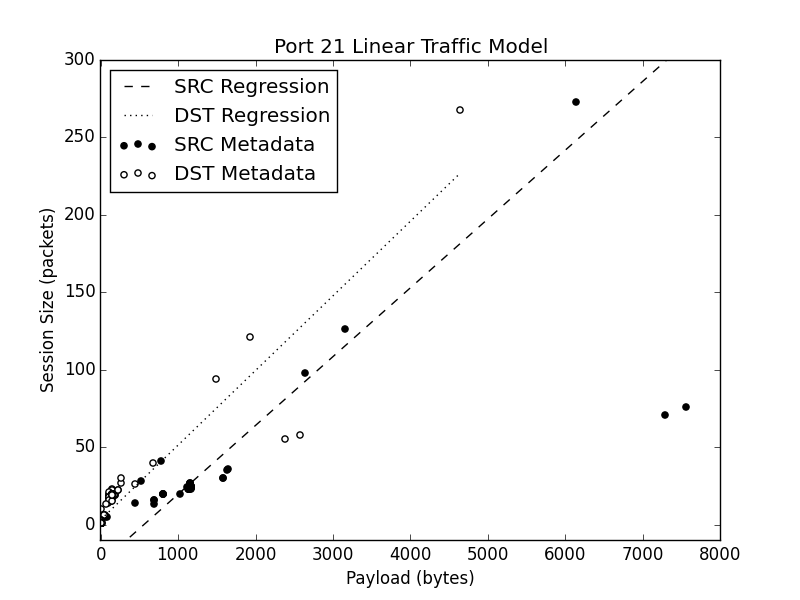
\includegraphics[width=9cm]{paperplots/21.png}
	\caption{FTP Traffic Model (1 min Snapshot)}
	\label{fig:21}
\end{figure}

Port 21, associated with File Transfer Protocol (FTP), has higher classification performance as a source (when the server is responding) versus the destination (when the client is sending). This is due to the nature of FTP, where server responses (port 21 as the source) are short and convey connection state information back to the client. Table \ref{tab:direction} has been provided for illustrative purposes of directional semantics. By nature, we would expect this traffic to have generalizable linear characteristics simply due to the fact a machine is the source of this traffic, and we believe this holds up in our analysis (see Figure \ref{fig:21}).

\begin{figure}[!htb]
	\centering
	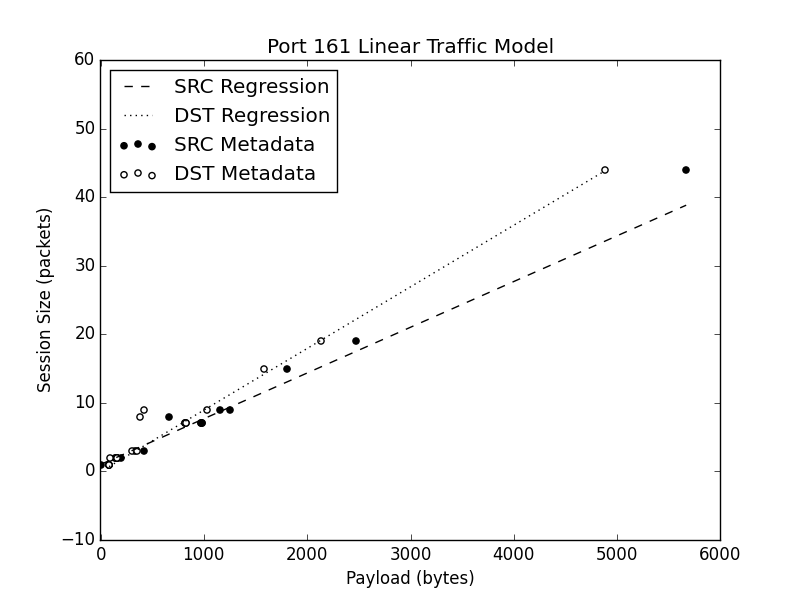
\includegraphics[width=9cm]{paperplots/161.png}
	\caption{SNMP Traffic Model (1 min Snapshot)}
	\label{fig:161}
\end{figure}

\begin{figure}[!htb]
	\centering
	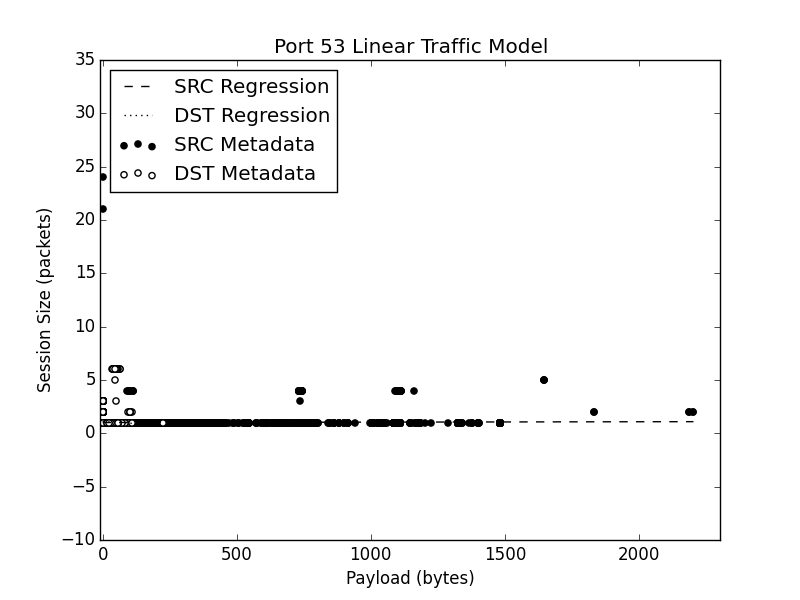
\includegraphics[width=9cm]{paperplots/53.png}
	\caption{DNS Traffic Model (1 min Snapshot)}
	\label{fig:53}
\end{figure}

Similarly, the same can be said of Port 161 (seen in Figure \ref{fig:161}), associated with Simple Network Management Protocol (SNMP) facilitating management of devices on a network by collecting data as well as changing device configuration information, as well as Domain Name Service (DNS) traffic on Port 53 (Figure \ref{fig:53}) resolving domain IP addresses. Given the preponderance of machine-generated traffic, behaving semi-deterministically, there lies a strong possibility for performing such network characterization to identify malicious traffic attempting to masquerade in this linear space \cite{7033254}.





However nondeterministic, user-based traffic is not necessarily out of reach from this effort. Figure \ref{fig:80} and \ref{fig:443} represent a one minute snapshot of unencrypted web traffic and both encrypted web and VPN traffic respectively. Although the intermediate model looks promising, the performance of Port 80 was 18.65\% on source traffic and 0.95\% on destination traffic, considerably lower than the top 10 in Table \ref{t:accuracy}. The disparity is due to the scale of the session payloads and the volume of traffic. Overall, web traffic (both encrypted and unencrypted) is a preponderance of the data, 99\% of which falling between 0-93kb in size and 1-71 packets in length. While this poses problems in terms of linear differentiability, we believe this could be overcome using hierarchical approaches.

Performing linear regression by applying the same technique on unique IP pairs within port 80 and 443 traffic adds another layer of behavioral characterization that can be captured. As an illustrative example, unencrypted UDP traffic originating from \texttt{espn.com} comprising of streaming video content would have a significantly different profile and patten to that of unencrypted TCP traffic from \texttt{bbc.com}. Likewise, encrypted UDP video traffic from \texttt{youtube.com} would have a different linear footprint than that of a standard search on \texttt{google.com}.

\begin{figure}[!htb]
	\centering
	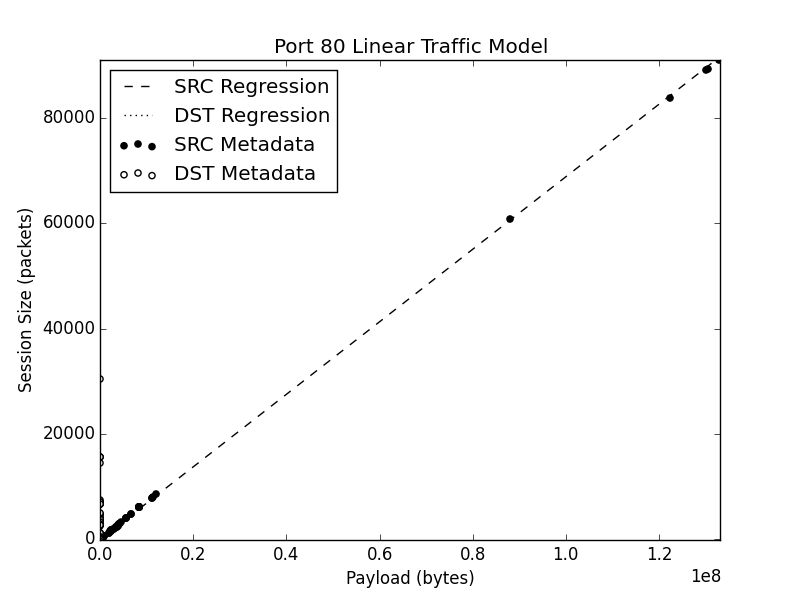
\includegraphics[width=9cm]{paperplots/80.png}
	\caption{Unencrypted Web Traffic Model (1 min Snapshot)}
	\label{fig:80}
\end{figure}

\begin{figure}[!htb]
	\centering
	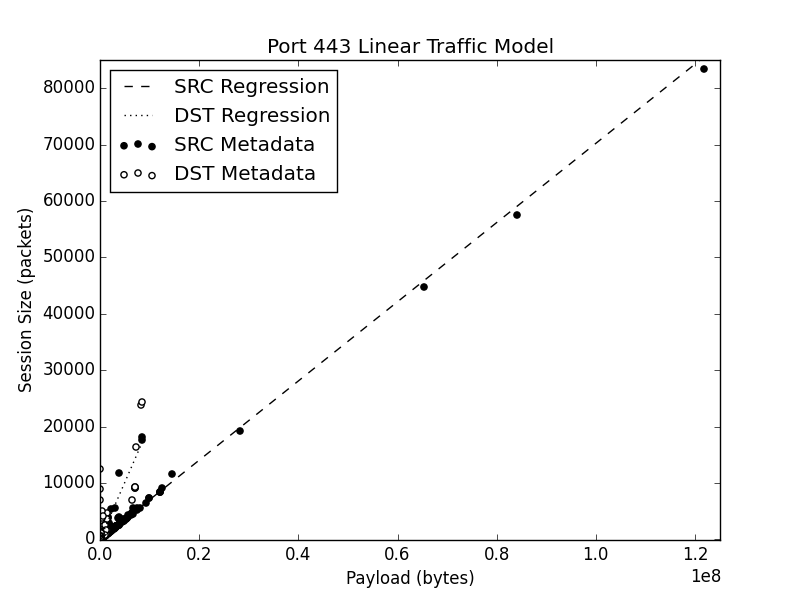
\includegraphics[width=9cm]{paperplots/443.png}
	\caption{Encrypted Web/VPN Traffic Model (1 min Snapshot)}
	\label{fig:443}
\end{figure}



\section{Future Work}
This work presents itself as the first step in the hierarchy of models for network traffic classification in order to ultimately normalize the every-day activity on the network and present a relative baseline to network security professionals.

Implementing the hierarchical classification system in order to increase linear differentiability will be a point of future work due to time constraints in this project. This would include a decomposition of port 80 and 443 traffic by unique IP pair, and implementing a distance metric in order to determine the appropriate depth within the hierarchy of classification models/mechanisms.

We are also keenly interested in the incorporation non-linear models within the hierarchical scheme in order to broaden the types of traffic flows that may be described \cite{PALMIERI2010737}. A similar exploratory phase of the feature space would need to be conducted in order to identify other data points to leverage.

Additionally, this work ultimately is to inform the construction of a detection system with the goal to identify conspicuous network traffic on well-known port numbers exhibiting linear features that of another port. A testing phase would undoubtedly include generating various sets of labeled network traffic (encrypted, unencrypted, varied port numbers and payload sizes) with desired features for system testing.

\section{Conclusion}
We have demonstrated the utility in using simple linear regression models in order to classify and characterize the behaviors of well-known port traffic, and discussed how the approach can be incorporated into a detection system utilizing a hierarchy of models (linear and non-linear) for use in capturing suspicious network flows.

\section{Acknowledgement}
Special thanks to Dr. Tingjian Ge for allowing me to pursue this work and to Dr. Chad Meiners as well as Dr. Dennis Ross for guidance and direction.

\begin{figure*}
	\centering
	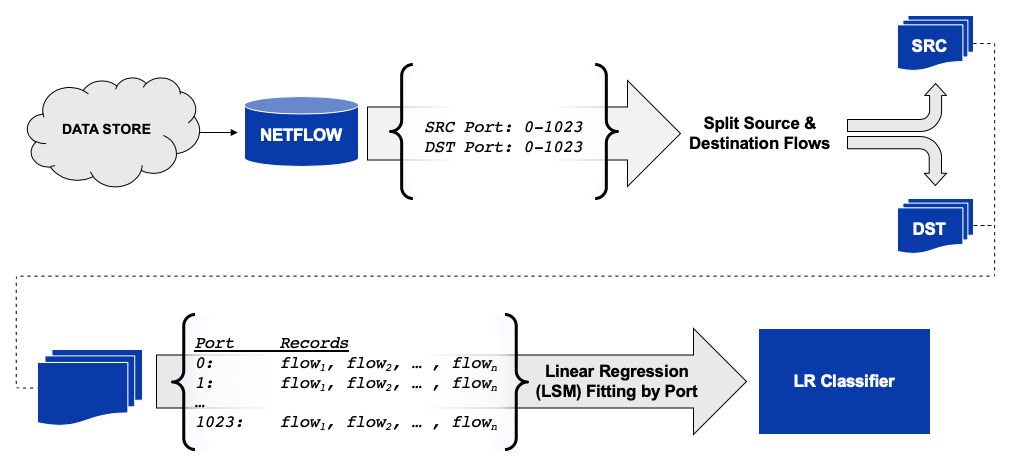
\includegraphics[width=15cm]{paperplots/process.png}
	\caption{Dataset creation and processing pipeline}
	\label{fig:processing}
\end{figure*}

\begin{figure*}
	\centering
	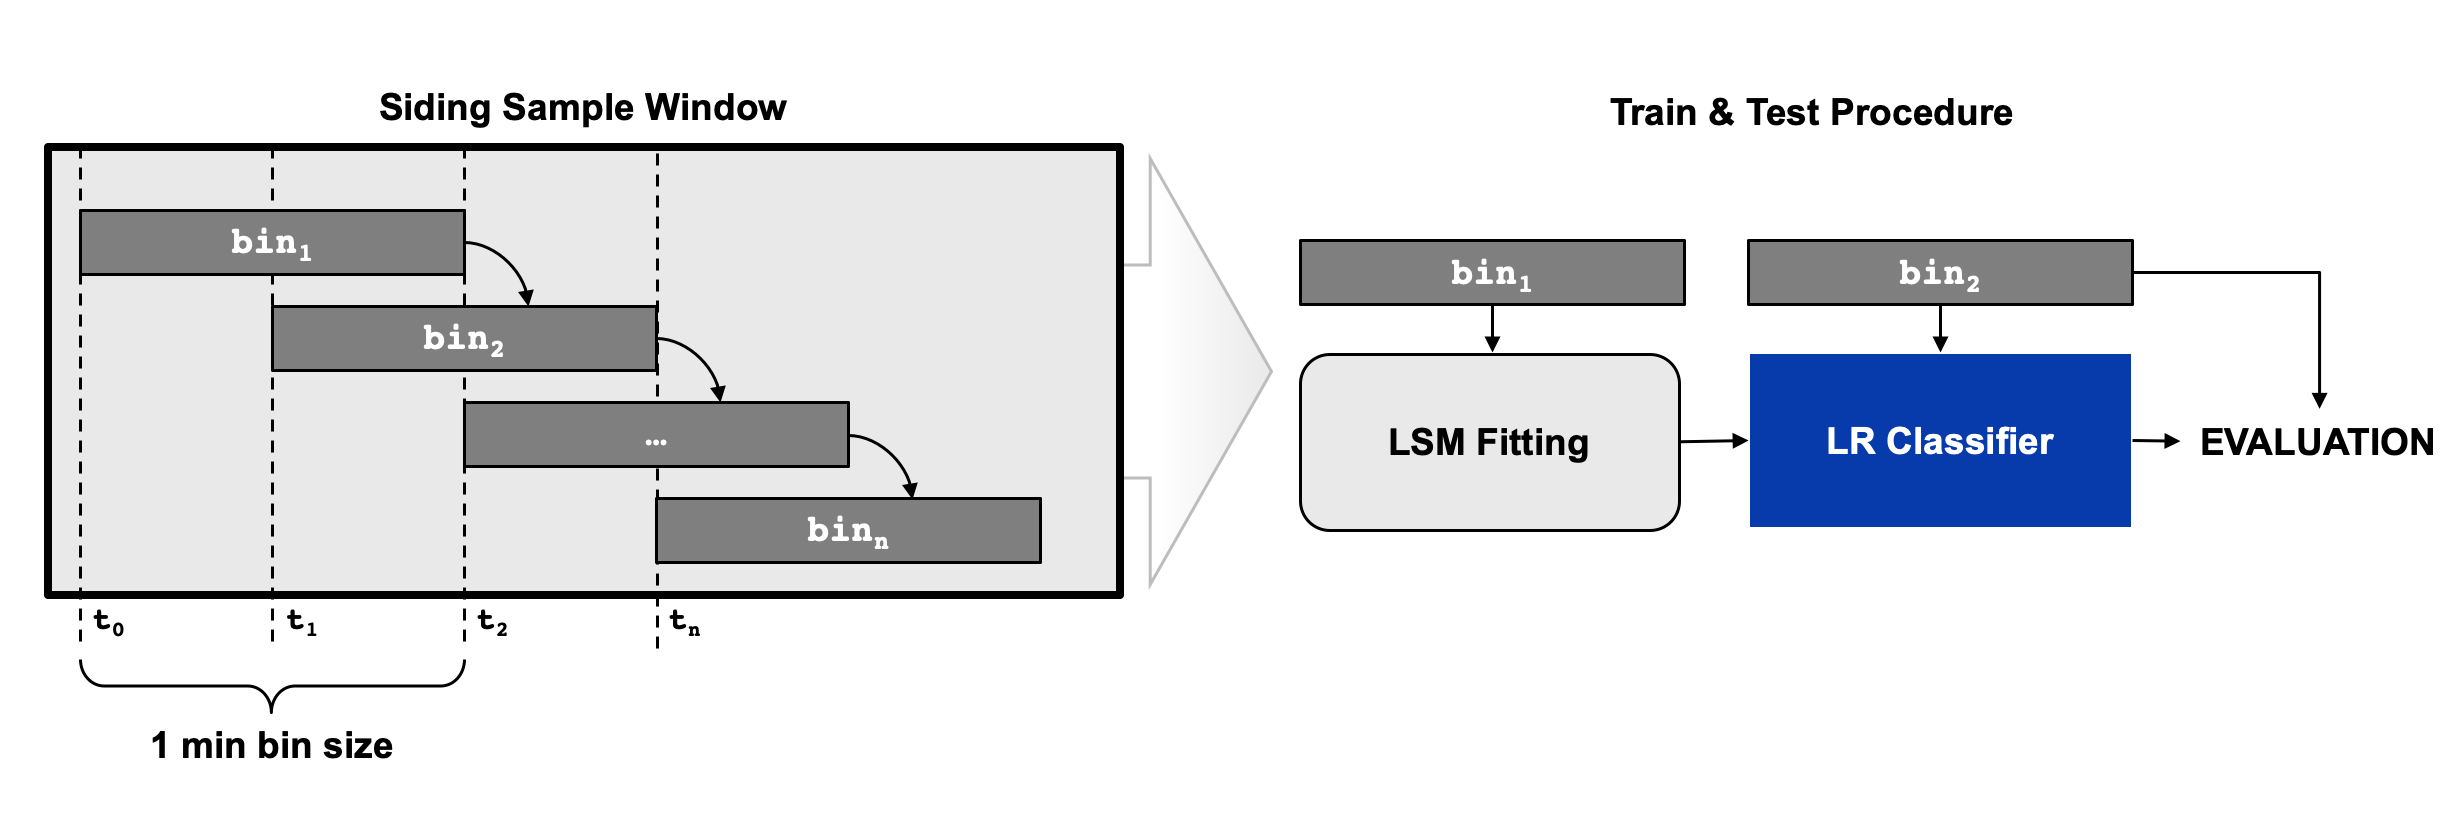
\includegraphics[width=15cm]{paperplots/model.png}
	\caption{Model batch-training and testing with ephemeral memory}
	\label{fig:model}
\end{figure*}


\bibliography{citations}
\bibliographystyle{ieeetr}

\end{document}
